\begin{minipage}[t]{180mm}
\fcolorbox{black}{white}{
\begin{minipage}[b]{30mm}

\includegraphics[width=0.5\linewidth]{unflogo.pdf}
\end{minipage}
\begin{minipage}[b]{100mm}
\Huge \textbf{UNF NEWZ} \\
\Large -- Søvn og retsstavning er overvurderet! 
\end{minipage}
\begin{minipage}[b]{50mm}
\Large Onsdag 17.07.2015 \\
\normalsize Redigeret i \LaTeX\ af \\ SOM, MGS, MMN, SABH
\end{minipage}
}
\end{minipage}



\begin{minipage}[b]{0.95\linewidth}
\begin{minipage}[t]{0.47\textwidth}
\vspace{3mm}
\section*{Brandbelæring}
Vi er blevet gjort opmærksom på, at den brandbelæring deltagerne modtog søndag ikke var fyldestgørende, så derfor kommer der her en mere udførlig brandbelæring: I tilfælde af mindre brand på instituttet skal Auditorium E forlades gennem nødudgangene og alle skal samle sig på græsplænen. Såfremt branden viser sig at være større, vil også denne plæne skulle forlades, og vi samles i stedet på pladsen overfor Statsbiblioteket. I tilfælde af at branden vokser sig større, specielt hvis den skulle gribe over til kemi, er dette sted på randen af Universitetsparken, dog lidt for tæt på, og vi vil derfor i stedet samle os på Østbanetorvet, hvilket ved endnu større brande, for eksempel i Fysiks accelerator, også gør det lettere at forlade byen ad sø- eller landvejen. Skulle branden skyldes krigeriske handlinger, specielt med fissionsvåben, anbefales det at Jylland forlades omgående. Til dette formål er der flere mulige router: Det letteste er måske at tage en båd fra havnen, dette ville dog kræve adgang og tilsvarende færdigheder. Da dette ikke kan forventes af alle deltagere på campen, er en anden mulighed at forlade byen til fods, enten mod nord, eventuel for at nå færger til Sverige eller Norge, eller mod Syd for at nå den tyske grænse. En flugt over land mod vest kan ikke umiddelbart anbefales, da dette kun ville åbne muligheden for at tage færgen fra Esbjerg mod de britiske øer. Skulle vi komme ud for, at der også vil blive anvendt fusionsvåben, anbefaler vi desuden at hele kontinentet forlades. Dette kan klares ved at vandre mod øst, og krydse Uralbjergene, hvilket vil være hård, men give mulighed for en ny tilværelse i Asiens stepper. Desuden kunne det prøves at krydse Middelhavet eller Atlanten på tømmerflåder eller i mindre både. Skulle dette overleves ville der være mulighed for en fortsat eksistens i Afrika eller på de Amerikanske dobbeltkontinent. På denne tid af året, vil pakisen omkring nordpolen sandsynligvis ikke være stabil nok til at gå til Grønland eller Canada, så denne rute anbefales kun til nøds. Desværre er der en vis risiko for total biologisk udslettelse af alle højere livsformer på jorden, denne kan vi dog også håndtere, ved, ad ovenstående ruter, at bevæge os til Bajkonur (eller til nøds Cape Canaverel), bortføre et rumskib, og flytte til ISS eller Månen. Hvis der derimod er tale om fysisk udslettelse af jordkloden, må dette forventes ikke at være nok, og der tilrådes derfor hurtigst muligt at udvikle den nødvendige teknologi for en envejsrejse til Mars. Nu burde alle menneskeskabte eventualiteter være afklaret, men vi bør også være forberedt på solens udslettelse, da denne ville medføre visse problemer for campens gennemførsel. I denne sammenhæng bør deltagere sende dem selv, helst i frosset tilstand, mod nære stjerner med formodede planeter, i håb om at kunne grundlægge en ny civilisation der. Desværre er denne strategi dog indtil videre begrænset på denne galaxe. Såfremt hele Mælkevejen udslettes, vil vi derfor skulle improvisere en effektiv løsning, hvilket de mere intelligente detagere sikkert sagtens kunne klare efter en kop medbragt kaffe eller to. Skulle det komme til Universets fulde destruktion, må vi stille større krav til deltagernes selvstændige overlevelsesevner, da dette kræver en duel med penne mod Platon i en velkendt restaurant, i hvilken sejren vil åbne en dør til idéernes verden, og fortsat eksistens i Eulers have med lov til at spise identiteten fra Cayleys træ.


\end{minipage}
\hfill\begin{minipage}[t]{0.47\textwidth}

\vspace{1mm}
\tikzstyle{mybox} = [draw=white, fill=blue!20, very thick,
    rectangle, rounded corners, inner sep=10pt, inner ysep=20pt]
\tikzstyle{fancytitle} =[fill=red, text=white]

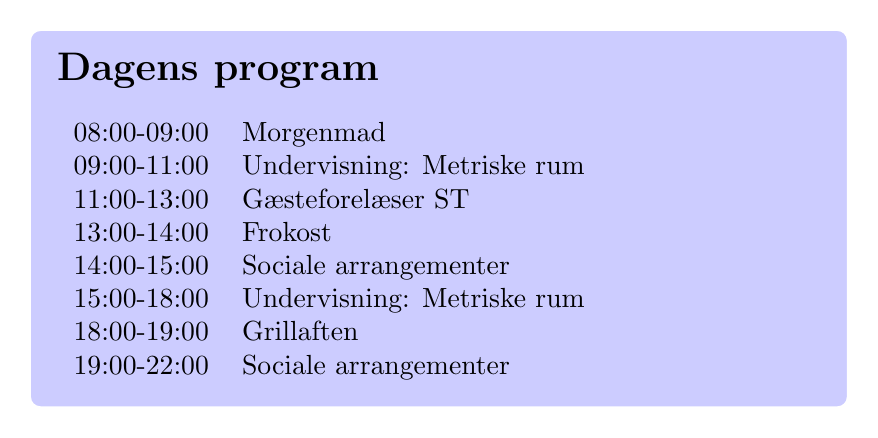
\begin{tikzpicture}
\node [mybox] (box){%
\begin{minipage}{0.80\textwidth}
\vspace{-4mm}\section*{Dagens program}
\begin{tabular}{ll}
08:00-09:00 & Morgenmad \\
09:00-11:00 & Undervisning: Metriske rum \\
11:00-13:00 & Gæsteforelæser ST \\
13:00-14:00 & Frokost \\
14:00-15:00 & Sociale arrangementer \\
15:00-18:00 & Undervisning: Metriske rum \\
18:00-19:00 & Grillaften \\
19:00-22:00 & Sociale arrangementer
\end{tabular}
\vspace{-4mm}
\end{minipage}
};
\end{tikzpicture}%
\vspace{-2mm}

\section*{Læserbrev: Skandale}

Kaere alle deltagere og arrangoerer paa dette aars camp!

Det er med stor sorg, at vi maa meddele, at grundet kommunikationsproblemer med campens oeverste ledelse, at vi ikke vil kunne deltage i dette aars camp. 
Det forholder sig saadan, at vi i oejeblikket befinder os i Sultan Hamengkoeboewono X's by, der i daglig tale kaldes Arhusaan paa det lokale sprog Bahasa Indonesia. 
Vi har beklagevis derfor faaet forvekslet denne by med Aarhus. Vi burde maaske have anet uraad, da Himmelbjerget her ligger nord for byen og eftersigende skulle vaere en meget aktiv vulkan! Men Jylland er jo et meget fremmed land for os Koebenhavnere/Fynboere, saa man ved jo aldrig helt, hvad man kan vente sig? Det er jo et udbredt faktum, at Jylland er lidt af et land i sig selv!
Vi maa derfor oenske jer alle en god camp og fortsat god sommer!

Mvh.Ann-Sofie (eks-Fysikcampkoordinator) og Sebastian (eks-Matematikcampkoordinator)

En kort vejudsigt her til sidst: meget varmt og solrigt, dog lidt skyer hen paa dagen og med lidt held en svag koelende brise.

PS. Husk ikke at spise om dagen i loebet af Ramadahen!

\vspace{2mm}


\includegraphics[width=\linewidth]{suprise.jpg}

\vspace{-4mm}
\section*{Pile konkurrence}
Det er kommet UNF Newz for øre, at der er startet en jagt på Campens pile. UNF newz kan sige, at der er ialt 70 pile / skilte der kan findes. \\
Denne konkurrence er et spørgsmål om ære, ikke om materialistisk vinding. Find pilene og marker dit fund (Dog uden at ødelægge pilens funktion), giv ære og respekt til dem der har fundet den før dig, og mærken den når andre finder pilene efter dig!

\end{minipage}
\end{minipage}
